% !TEX root = ../../../main.tex
% 来源：中学数学实验教材·第一册（代数）
% 章节：因式分解与余式定理 / 辗转相除法
% 原始文件：5.tex，行 2397-2446
% 类型：tikz
% ---
    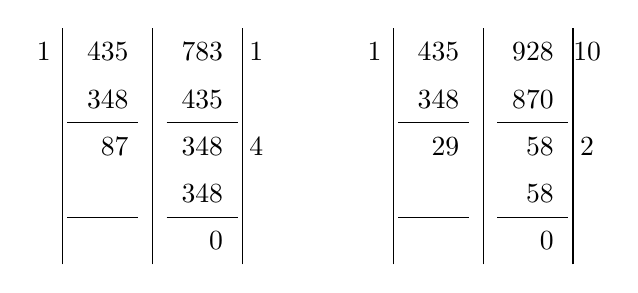
\begin{tikzpicture}[scale=.6]
    \begin{scope}
\foreach \y/\ytext in {0/{},1/{},2/\boxed{87},3/348,4/435}
{
    \node at (-1, \y)[left]{$\ytext$};
}    
\foreach \y/\ytext in {0/0,1/348,2/348,3/435,4/783}
{
    \node at (1, \y)[left]{$\ytext$};
}   
\foreach \x in {-2.6,-.7,1.2}
{
    \draw (\x,-.5)--(\x,4.5);
}

\foreach \y in {.5, 2.5}
{
    \draw (-2.5,\y)--(-1,\y);
    \draw (-.4,\y)--(1.1,\y);
}
\node at (-3, 4) {1};
\node at (1.5, 4) {1};
\node at (1.5, 2) {4};      
    \end{scope}


    \begin{scope}[xshift=7cm]
\foreach \y/\ytext in {0/{},1/{},2/\boxed{29},3/348,4/435}
{
    \node at (-1, \y)[left]{$\ytext$};
}    
\foreach \y/\ytext in {0/0,1/58,2/58,3/870,4/928}
{
    \node at (1, \y)[left]{$\ytext$};
}   
\foreach \x in {-2.6,-.7,1.2}
{
    \draw (\x,-.5)--(\x,4.5);
}

\foreach \y in {.5, 2.5}
{
    \draw (-2.5,\y)--(-1,\y);
    \draw (-.4,\y)--(1.1,\y);
}
\node at (-3, 4) {1};
\node at (1.5, 4) {10};
\node at (1.5, 2) {2};
    \end{scope}    
\end{tikzpicture}   
